\documentclass[a4paper, 11pt]{article}
\usepackage{comment}
\usepackage{lipsum} 
\usepackage{fullpage} %cambiar margen
\usepackage[a4paper, total={7in, 10in}]{geometry}

\usepackage{amssymb,amsthm} 
\usepackage{amsmath}
\newtheorem{theorem}{Theorem}
\newtheorem{corollary}{Corollary}
\usepackage{graphicx}
\usepackage{tikz}
\usetikzlibrary{arrows}
\usepackage{verbatim}
%\usepackage[numbered]{mcode}
\usepackage{float}
\usepackage{tikz}
\usetikzlibrary{shapes,arrows}
\usetikzlibrary{arrows,calc,positioning}
\usepackage{mathpazo} %tipo de letra 
\usepackage[utf8]{inputenc} %codificación
\usepackage[T1]{fontenc} %digitación de tildes y ñ
\usepackage[spanish]{babel} %paquete de soporte español

\tikzset{
	block/.style = {draw, rectangle,
		minimum height=1cm,
		minimum width=1.5cm},
	input/.style = {coordinate,node distance=1cm},
	output/.style = {coordinate,node distance=4cm},
	arrow/.style={draw, -latex,node distance=2cm},
	pinstyle/.style = {pin edge={latex-, black,node distance=2cm}},
	sum/.style = {draw, circle, node distance=1cm},
}
\usepackage{xcolor}
\usepackage{mdframed}
\usepackage[shortlabels]{enumitem}
\usepackage{indentfirst}
\usepackage{hyperref}

\usepackage{listings}
\lstset{literate=
  {á}{{\'a}}1
  {é}{{\'e}}1
  {í}{{\'i}}1
  {ó}{{\'o}}1
  {ú}{{\'u}}1
  {Á}{{\'A}}1
  {É}{{\'E}}1
  {Í}{{\'I}}1
  {Ó}{{\'O}}1
  {Ú}{{\'U}}1
  {ñ}{{\~n}}1
  {ü}{{\"u}}1
  {Ü}{{\"U}}1
}

\lstdefinestyle{customc}{
  belowcaptionskip=1\baselineskip,
  breaklines=true,
  frame=L,
  xleftmargin=\parindent,
  language=Python,
  showstringspaces=false,
  basicstyle=\footnotesize\ttfamily,
  keywordstyle=\bfseries\color{green!40!black},
  commentstyle=\itshape\color{purple!40!black},
  identifierstyle=\color{blue},
  stringstyle=\color{orange},
}

\lstdefinestyle{customasm}{
  belowcaptionskip=1\baselineskip,
  frame=L,
  xleftmargin=\parindent,
  language=[x86masm]Assembler,
  basicstyle=\footnotesize\ttfamily,
  commentstyle=\itshape\color{purple!40!black},
}

\lstset{escapechar=@,style=customc}



\renewcommand{\thesubsection}{\thesection.\alph{subsection}}

\newenvironment{problem}[2][Ejercicio]
{ \begin{mdframed}[backgroundcolor= red!50] \textbf{#1 #2} \\}
	{  \end{mdframed}}

% Define solution environment
\newenvironment{solution}
{\textcolor{blue}{\textbf{\textit{Solución:\\\noindent}}}}


\renewcommand{\qed}{\quad\qedsymbol}

% \\	
\begin{document}
	\noindent
	%%%%%%%%%%%%%%%%%%%%%%%%%%%%%%%%%%%%
	
	\begin{minipage}[b][1.2cm][t]{0.8\textwidth}
		\large\textbf{César Isaí García Cornejo} \hfill \textbf{Tarea 1}  \\
		cesar.cornejo@cimat.mx \hfill \\
		\normalsize Computo Científico \hfill Semestre 3\\
	\end{minipage}
	
	\hspace{14.4cm}
	\begin{minipage}[b][0.03cm][t]{0.12\linewidth}
		
		\vspace{-2.2cm}
		%%%La Ruta depeendera de donde este alojado el main y la imagen
		
\includegraphics[scale=0.3]{Figures/EscudoCimat.png}
	\end{minipage}
	
	\noindent\rule{7in}{2.8pt}
	
	%%%%%%%%%%%%%%%%%%%%%
	%%%%%%%%%%%%%%%%%%%%%%%%%%%%%%%%%%%%%%%%%%%%%%%%%%%%%%%%%%%%%%%%%%%%%%%%%%%%%%%%%%%%%%%%%%%%%%%%%%%%%%%%%%%%%%%%%%%
	% Problem 1
	%%%%%%%%%%%%%%%%%%%%%%%%%%%%%%%%%%%%%%%%%%%%%%%%%%%%%%%%%%%%%%%%%%%%%%%%%%%%%%%%%%%%%%%%%%%%%%%%%%%%%%%%%%%%%%%%%%%%%%%%%%%%%%%%%%%%%%%%
	\setlength{\parskip}{\medskipamount}
	\setlength{\parindent}{0pt}
 
\begin{problem}{1}
Implementar los algoritmos de \textit{Backward} y \textit{Forward substitution}.
\end{problem}

\begin{solution}

Para poder obtener un algoritmo que ejecute una \textbf{substitución \textit{forward}} es necesario un sistema de ecuaciones lineales
cuya matriz es triangular inferior. Es decir, el sistema se puede expresar de la forma
\begin{align}
    L y = b
\end{align}
donde L es una matriz triangular inferior. Otra forma de verlo es por medio de la expansión 
\begin{align*}
    \begin{pmatrix}
        l_{11} & 0 & 0 & \cdots  & 0 \\ 
        l_{21} & l_{22} &0 & \cdots  & 0 \\ 
        l_{31} & l_{32} & l_{33} & \cdots  & 0 \\ 
         \vdots & \vdots & \vdots & \ddots  & \vdots\\ 
         l_{m1}& l_{m2}  & l_{m3}& \cdots & l_{mm}
        \end{pmatrix}
        \begin{pmatrix}
        y_1\\ 
        y_2\\ 
        y_3\\
        \vdots \\ 
        y_m
        \end{pmatrix}
        =
        \begin{pmatrix}
        b_1\\ 
        b_2\\ 
        b_3\\
        \vdots \\ 
        b_m
        \end{pmatrix}        
\end{align*}

Así tenemos,
\begin{align}
    y_1 &= \frac{b_1}{l_{11}}, \nonumber\\
    y_2 &= \frac{b_2 -  l_{21} y_2 }{l_{22}},\nonumber\\
    &\vdots \nonumber \\
    y_j &= \frac{\left (b_j - l_{j1}y_1 -l_{j2}y_2 -\cdots-l_{j,j-1}y_{j-1} \right )}{l_{jj}}, \:\:\:\:\:\:\:\:\: 2 \leq j \leq m.
    \label{1.03}
\end{align}


Para la implementación de dicho algoritmo es necesario anidar dos ciclos for. Se crea una variable auxiliar llamada aux, la cual el ciclo for interno suma los terminos $l_{j1}y_1 +l_{j2}y_2 + \cdots + l_{j,j-1}y_{j-1}$ para posteriormente usar (\ref{1.03})

\begin{lstlisting}
for i in range(len(b)):
    aux = 0    
    for j in range(i):
        aux += L[i,j]*y[j]   #Auxiliar variable
    y[i] = (b[i] - aux)/L[i,i]   # 'y' is the output and solution to the system of equations.
\end{lstlisting}

Por otro lado, la implementación de la \textbf{ substitución \textit{backward}} es análogo al algoritmo previo. Consideremos el sistema de ecuaciones lineales
\begin{align}
    Ux = b
\end{align}
donde $U$ es una matriz triangular superior. La expansión es de la forma
\begin{align*}
    \begin{pmatrix}
        u_{11} & u_{12} & u_{13} & \cdots  & u_{1m} \\ 
        \vdots & \vdots & \vdots & \ddots  & \vdots\\ 
        0 &0 & u_{m-2,m-2} & u_{m-2,m-1}   & u_{m-2,m} \\
        0 & 0 &  0 &u_{m-1,m-1} & u_{m-1,m} \\
        0 & 0  & 0& 0 & u_{mm}
        \end{pmatrix}
        \begin{pmatrix}
        x_1\\ 
        \vdots \\
        x_{m-2}\\ 
        x_{m-1}\\ 
        x_m
        \end{pmatrix}
        =
        \begin{pmatrix}
        b_1\\ 
        \vdots \\ 
        b_{m-2}\\ 
        b_{m-1}\\
        b_m
        \end{pmatrix}  
\end{align*}

De esta forma
\begin{align}
    x_{mm} &= \frac{b_m}{u_{mm}}, \nonumber\\
    x_{m-1,m-1} &= \frac{b_{m-1} - u_{m-1,m}x_m}{u_{m-1,m-1}},\nonumber \\
    \vdots\nonumber\\
    x_{i,i} &= \frac{b_{m-1} - u_{i,m}x_m - u_{i,m-1}x_{m-1}-\cdots-u_{i,m-i-1}x_{m-i-1}}{u_{i,i}}
    \label{1.04}
\end{align}

La implementación del algoritmo para la substitución \textit{backward} es análago. La diferencia sustancial entre ambos se encuetra en que los indices de los vectores deben de correr al reves. Dicha implementación se fundamenta en el siguiente código.
\begin{lstlisting}
for i in range(m):
        aux = 0
        for j in range(i):
            aux += U[m-i-1,m-j-1] * x[m-j-1]      #Auxiliar variable
        x[m-i-1] = (b[m-i-1] - aux)/U[m-i-1,m-i-1]    # Form obtained by 'despeje' of the variable of interest.
\end{lstlisting}

Lo que completa la implementación de ambos métodos.

\end{solution}
	
\begin{problem}{2}
    Implementar el algoritmo de eliminación Gaussiana con pivoteo parcial LUP, 21.1 del Trefethen (p. 160).
\end{problem}
    
\begin{solution}
La implementación es directa del pseudocódigo. Sea $A$ una matriz numpy. Se crean tres matrices vacias (nulas) donde se almacenarán a L,U y P.

\begin{lstlisting}
U = A.copy()
L = np.identity(m,dtype= float)
P = np.identity(m,dtype= float)
\end{lstlisting}

Es importante resaltar que la matriz $U$ requiere ser una copia de A. Sin el metodo copy() el lenguage solamente haría referencia a la dirección de memoria y esta se modificaría.

La generalización de la factorización LU con pivoteo se sigue de una serie de modificaciones iterativas (cambios de renglos) dentro del primer for anidado. Es entonces que se pide encontrar el indice de la fila que hace que el valor k-ésimo de la columna se maximice. Esto se implementó con el siguiente código.

\begin{lstlisting}
    for k in range(m-1):

    Index_max = k
    maxi = U[k,k]

        for i in range(k, m):  #This cicle for stan for check the maximum of the k-column.
            if abs(U[i,k]) > abs(maxi):
                maxi = U[i,k]
                Index_max = i
\end{lstlisting}

Lo siguiente a realizar es un cambio de renglones en las matrices L,U y P. Los cambios de L y P son directos ya que se cambia todo el renglon. Sin embargo, los cambios de L son más delicados pues solo se cambia una parte de cada renglon. Esto con el código siguiente:
\begin{lstlisting}
    AuxRowL = L[k,: k].copy()
    L[k,: k] = L[Index_max,: k]
    L[Index_max,: k] = AuxRowL
\end{lstlisting}

Posteriormente se finaliza el método al anidar el segundo ciclo for mismo que en la factorización LU convencional. Los detalles se encuentra en el script adjunto.

\end{solution}

\begin{problem}{3}
    Dar la descomposición LUP para una matriz aleatoria de entradas U(0,1) de tamaño 5$\times 5$, y para la matriz
    \begin{align}
        A = \begin{pmatrix}
            1 &0  &0  &0 &1 \\ 
            -1 &1  &0  &0 &1 \\ 
            -1 &-1  &1 &0  &1 \\ 
            -1 &-1  &-1  &1 &1\\
            -1 & -1 & -1 & -1 &1 
            \end{pmatrix}
    \label{1.07}
    \end{align}
\end{problem}

\begin{solution}    

Para la matriz dada, se manda a llamar la función $LUP(A)$ donde la matriz A es la función a factorizar.

El resultado de la descomposición $PA = LU$ es
\begin{align}
    A
    =
    \begin{bmatrix}
        1. & 0. & 0. & 0. & 0.\\
        -1. & 1. & 0. & 0. & 0.\\
        -1. & -1. & 1. & 0. & 0.\\
        -1. & -1. & -1. & 1. & 0.\\
        -1. & -1. & -1. & -1. & 1.\\
      \end{bmatrix}
      \begin{bmatrix}
        1. & 0. & 0. & 0. & 1.\\
        0. & 1. & 0. & 0. & 2.\\
        0. & 0. & 1. & 0. & 4.\\
        0. & 0. & 0. & 1. & 8.\\
        0. & 0. & 0. & 0. & 16.\\
      \end{bmatrix}
\end{align}
donde para este caso particular $P$ es la matriz identidad.

Usando la paqueteria de Scipy, se implementó el generador de matrices y vectores con entradas aleatorios con distribución uniforme (0,1). Además, se ajusto una \textit{semilla} para mayor control de la matriz aleatoria. La matriz generada es:
\begin{align*}
    D =
    \begin{bmatrix}
        0.15416284 & 0.7400497 & 0.26331502 & 0.53373939 & 0.01457496\\
        0.91874701 & 0.90071485 & 0.03342143 & 0.95694934 & 0.13720932\\
        0.28382835 & 0.60608318 & 0.94422514 & 0.85273554 & 0.00225923\\
        0.52122603 & 0.55203763 & 0.48537741 & 0.76813415 & 0.16071675\\
        0.76456045 & 0.0208098 & 0.13521018 & 0.11627302 & 0.30989758\\
      \end{bmatrix}
\end{align*}
Su descomposición LU es tal que
\begin{align*}
    P &=
    \begin{bmatrix}
        0. & 1. & 0. & 0. & 0.\\
        0. & 0. & 0. & 0. & 1.\\
        0. & 0. & 1. & 0. & 0.\\
        1. & 0. & 0. & 0. & 0.\\
        0. & 0. & 0. & 1. & 0.\\
      \end{bmatrix},\\
      L &= \begin{bmatrix}
        1. & 0. & 0. & 0. & 0.\\
        0.83217735 & 1. & 0. & 0. & 0.\\
        0.30892983 & -0.44984958 & 1. & 0. & 0.\\
        0.16779684 & -0.80811921 & 0.35073561 & 1. & 0.\\
        0.56732269 & -0.05631829 & 0.48102103 & -0.24994986 & 1.\\
      \end{bmatrix},\\
      U &= \begin{bmatrix}
        0.91874701 & 0.90071485 & 0.03342143 & 0.95694934 & 0.13720932\\
        0. & -0.7287447 & 0.10739762 & -0.68007855 & 0.1957151\\
        0. & 0. & 0.98221304 & 0.2511723 & 0.04791354\\
        0. & 0. & 0. & -0.26451328 & 0.13290782\\
        0. & 0. & 0. & 0. & 0.10407\\
      \end{bmatrix}
\end{align*}

lo que concluye el ejercicio.

\end{solution}

\begin{problem}{4}
    Usando la descomposición LUP anterior, resolver el sistema de la forma
    \begin{align}
        Dx = b 
    \end{align}
    donde $D$ son las matrices del problema 3, para 5 diferentes $b$ aleatorios con entradas $U(0,1)$. Verificando si es posible o no resolver el sistema.
\end{problem}

\begin{solution}
Para resolver el sisteme $Ax = b$ con el método de descomposición LU con pivoteo necesitamos hacer manipulaciones algebraicas. Notemos que
\begin{align*}
    A x &= b,\\
    PA x &= Pb,\\
    LU x &= Pb,\\
    L y &= Pb,\\
    \intertext{donde}
    U x &= y 
\end{align*}
Por tanto, es necesario resolver con \textit{backward substitution} para obtener $y$, luego con \textit{forward substitution} se puede resolver para x. Esto siempre y cuando el sistema tenga solución única.

La función definida en el script, a manera de sumario es
\begin{lstlisting}
def LinearSystem(A,b):
    try:   
        L,U,P = LUP(A)

        y = forward(L,P@b)
        x = backward(U,y)
    except:
        print("The system of equations do not have a unique solution")
        
    return x
\end{lstlisting}
que intenta resolver el sistema por medio de la factorización LU con pivoteo. Si se da el caso de que la matriz es degenerada o cercana a una degenerada, entonces saltará un error e imprimirá que no hay solución.

Debido a que son 5 vectores b aleatorios, solo presentaremos uno y el resto se podrán obtener tras compilar el código correspondiente.

Para el sistema $Ax = b$
\begin{align*}
    \begin{bmatrix}
        1. & 0. & 0. & 0. & 1.\\
        -1. & 1. & 0. & 0. & 1.\\
        -1. & -1. & 1. & 0. & 1.\\
        -1. & -1. & -1. & 1. & 1.\\
        -1. & -1. & -1. & -1. & 1.\\
      \end{bmatrix}
      \begin{bmatrix}
        x_{1} \\x_{2} \\ x_{3} \\ x_{4} \\ x_{5}\\
      \end{bmatrix} = 
      \begin{bmatrix}
        0.15416284 \\ 0.7400497 \\ 0.26331502 \\ 0.53373939 \\ 0.01457496\\
      \end{bmatrix}
\end{align*}
donde la solución es dada por
\begin{align*}
    \begin{bmatrix}
        x_{1} \\x_{2} \\ x_{3} \\ x_{4} \\ x_{5}\\
    \end{bmatrix} =\begin{bmatrix}
        -0.17511503 \\ 0.2356568 \\ -0.00542108 \\ 0.25958222 \\ 0.32927787\\
    \end{bmatrix}
\end{align*}

Para matrices aleatorias funciona igual.

\end{solution}

\begin{problem}{5}
    Implementar el algoritmo de descomposición de Cholesky 23.1 del Trefethen (p. 175).
\end{problem}

\begin{solution}
    
La descomposición de Cholesky funciona exclusivamente para matrices hermitianas (simétricas) y positivas definidas. Consideremos la matriz A y construyamos una matriz con las carácteristicas anteriormente mencionadas. Tomemos $D =A^*A$. Es claro que $D*= A^* A$, es decir $D^* = D$ una matriz hermitiana. Luego tomemos un vector $x \in \mathbb{C}^m $
e investiguemos 
\begin{align*}
    x^* D x &= x^* A^*A x,\\
    &= (Ax)^* Ax,\\
    &= ||Ax||^2 \geq 0
\end{align*}
para $x \neq 0$ define una matrix definida positiva.

La implementación es directa del pseudocódigo. A manera de sumario:
\begin{lstlisting}
def cholesky(D):
    
    import numpy as np
    R = D.copy()
    m = np.shape(D)[0]

    for k in range(m):
        for j in range(k+1,m):
            
            R[j,j:] = R[j,j:] - R[k,j:] * (R[k,j]/R[k,k])

        R[k,k:] = R[k,k:]/np.sqrt(R[k,k])
\end{lstlisting}

debido a que el algoritmo reescribe sobre la matriz R, entonces la diagonal inferor debería anularse por lo que es necesario construir un algoritmo para la limpia de dicho R. Esto simpliemente con el comando
\begin{lstlisting}
    for i in range(m):
        for j in range(i):
            R[i,j] = 0
\end{lstlisting}
que anula cada elemento debajo de la identidad.

Usando la matrix (\ref{1.07}) podemos construir de la forma ya mencionada la matriz de entrada a Cholesky. La matriz $D$ es
\begin{align*}
    D = \begin{bmatrix}
        5. & 2. & 1. & 0. & -3.\\
        2. & 4. & 1. & 0. & -2.\\
        1. & 1. & 3. & 0. & -1.\\
        0. & 0. & 0. & 2. & 0.\\
        -3. & -2. & -1. & 0. & 5.\\
      \end{bmatrix}
\end{align*}
cuya factorización es $D = R^* R$ con 
\begin{align*}
    R = \begin{bmatrix}
        2.23606798 & 0.89442719 & 0.4472136 & 0. & -1.34164079\\
        0. & 1.78885438 & 0.3354102 & 0. & -0.4472136\\
        0. & 0. & 1.63935963 & 0. & -0.15249857\\
        0. & 0. & 0. & 1.41421356 & 0.\\
        0. & 0. & 0. & 0. & 1.72532437\\
      \end{bmatrix}
\end{align*}
lo que concluye la implementación.

\end{solution}



\begin{problem}{6}
    Comparar la complejidad de su implementación de los algoritmos de factorización de Cholesky y LUP mediante la medición de los tiempos que tardan con respecto a la descomposición de una matriz aleatoria hermitiana definida positiva. Graficar la comparación.
\end{problem}

\begin{solution}
    
Mediante la paquetería time podemos medir la \textit{hora} en nanoseundos. Ahora buscamos medir el tiempo de ejecución de un programa en función del tamaño de la matriz de entrada para cada uno de los dos métodos de factorización vistos. 

Con el código podemos guardar el resultado del tiempo de ejecución
\begin{lstlisting}

inicio = time.time()
LUP(A)
fin = time.time()

tiempoLU[i] = fin - inicio
\end{lstlisting}
para el caso de LUP. El caso Cholesky es similar. Luego graficamos dichos tiempos para matrices que van desde $\mathbb{R}^{1\times 1}$ hasta $\mathbb{R}^{600 \times 600}$ 

\begin{figure}[H]
    \centering
    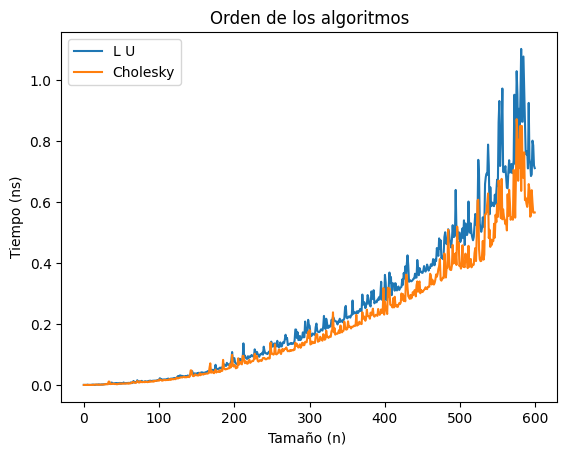
\includegraphics[width = 13 cm]{Figures/output2.png}
    \caption{Tiempo de ejecución de los métodos de factorización LU y Cholesky}
\end{figure}

Observemos que ambos procesos parecen tener el tiempo creciente de orden polinomial. También podemos notar que el método LU es mas complejo pues usa mas operaciones que el método de Cholesky.








\end{solution}


\end{document}